
\documentclass[xcolor=dvipsnames]{beamer}
\usecolortheme[named=MidnightBlue]{structure}
\setbeamertemplate{items}[ball]
\setbeamertemplate{blocks}[rounded][shadow=true]

\usetheme{Warsaw}
\useoutertheme[subsection=false]{smoothbars}


% include packages
\usepackage{multicol}
\usepackage{amsmath}
\usepackage{epsfig}
\usepackage{graphicx}
\usepackage[all,knot]{xy}
\xyoption{arc}
\usepackage{url}
\usepackage{multimedia}
\usepackage{hyperref}
\usepackage[autostyle]{csquotes}
\newenvironment<>{proofs}[1][\proofname]{%
    \par
    \def\insertproofname{#1{.}}%
    \usebeamertemplate{proof begin}#2}
  {\usebeamertemplate{proof end}}
\newenvironment<>{proofc}{%
  \setbeamertemplate{proof begin}{\begin{block}{}}
    \par
    \usebeamertemplate{proof begin}}
  {\usebeamertemplate{proof end}}
\newenvironment<>{proofe}{%
    \par
    \pushQED{\qed}
    \setbeamertemplate{proof begin}{\begin{block}{}}
    \usebeamertemplate{proof begin}}
  {\popQED\usebeamertemplate{proof end}}
\makeatother

%norm, absolute value commands
\newcommand{\norm}[1]{\left|\left|#1\right|\right|}
\newcommand{\abs}[1]{\left|#1\right|}
%curl and div commands
\newcommand{\curl}{\nabla\times}
\renewcommand{\div}{\nabla\cdot}
%better Re and Im commands
\renewcommand{\Re}{\text{Re}}
\renewcommand{\Im}{\text{Im}}
%new QED symbol
\renewcommand{\qedsymbol}{\textcolor{RedViolet}{$\blacksquare$}}
%approximately less/greater than
\newcommand{\approxleq}{\tiny{ \raisebox{-0.3ex}{$\,\stackrel{\raisebox{-.2ex}{$\textstyle <$}}{\sim}\,$}} }
\newcommand{\approxgeq}{\tiny{ \raisebox{-0.3ex}{$\,\stackrel{\raisebox{-.2ex}{$\textstyle >$}}{\sim}\,$}} }
\newcommand{\al}{\alpha} %Steal ALL of Dr. Kable's Aliases! MWAHAHAHAHA!
\newcommand{\be}{\beta}
\newcommand{\ga}{\gamma}
\newcommand{\Ga}{\Gamma}
\newcommand{\de}{\delta}
\newcommand{\De}{\Delta}
\newcommand{\ep}{\epsilon}
\newcommand{\vep}{\varepsilon}
\newcommand{\ze}{\zeta}
\newcommand{\et}{\eta}
\newcommand{\tha}{\theta}
\newcommand{\vtha}{\vartheta}
\newcommand{\Tha}{\Theta}
\newcommand{\io}{\iota}
\newcommand{\ka}{\kappa}
\newcommand{\la}{\lambda}
\newcommand{\La}{\Lambda}
\newcommand{\rh}{\rho}
\newcommand{\si}{\sigma}
\newcommand{\Si}{\Sigma}
\newcommand{\ta}{\tau}
\newcommand{\ups}{\upsilon}
\newcommand{\Ups}{\Upsilon}
\newcommand{\ph}{\phi}
\newcommand{\Ph}{\Phi}
\newcommand{\vph}{\varphi}
\newcommand{\vpi}{\varpi}
\newcommand{\ch}{\chi}
\newcommand{\ps}{\psi}
\newcommand{\Ps}{\Psi}
\newcommand{\om}{\omega}
\newcommand{\Om}{\Omega}

\newcommand{\bbA}{\mathbb{A}}
\newcommand{\A}{\mathbb{A}}
\newcommand{\bbB}{\mathbb{B}}
\newcommand{\bbC}{\mathbb{C}}
\newcommand{\C}{\mathbb{C}}
\newcommand{\bbD}{\mathbb{D}}
\newcommand{\bbE}{\mathbb{E}}
\newcommand{\bbF}{\mathbb{F}}
\newcommand{\bbG}{\mathbb{G}}
\newcommand{\G}{\mathbb{G}}
\newcommand{\bbH}{\mathbb{H}}
\newcommand{\HH}{\mathbb{H}}
\newcommand{\bbI}{\mathbb{I}}
\newcommand{\I}{\mathbb{I}}
\newcommand{\bbJ}{\mathbb{J}}
\newcommand{\bbK}{\mathbb{K}}
\newcommand{\bbL}{\mathbb{L}}
\newcommand{\bbM}{\mathbb{M}}
\newcommand{\bbN}{\mathbb{N}}
\newcommand{\N}{\mathbb{N}}
\newcommand{\bbO}{\mathbb{O}}
\newcommand{\bbP}{\mathbb{P}}
\newcommand{\PP}{\mathbb{P}}
\newcommand{\bbQ}{\mathbb{Q}}
\newcommand{\Q}{\mathbb{Q}}
\newcommand{\bbR}{\mathbb{R}}
\newcommand{\R}{\mathbb{R}}
\newcommand{\bbS}{\mathbb{S}}
\newcommand{\bbT}{\mathbb{T}}
\newcommand{\bbU}{\mathbb{U}}
\newcommand{\bbV}{\mathbb{V}}
\newcommand{\bbW}{\mathbb{W}}
\newcommand{\bbX}{\mathbb{X}}
\newcommand{\bbY}{\mathbb{Y}}
\newcommand{\bbZ}{\mathbb{Z}}
\newcommand{\Z}{\mathbb{Z}}

\newcommand{\scrA}{\mathcal{A}}
\newcommand{\scrB}{\mathcal{B}}
\newcommand{\scrC}{\mathcal{C}}
\newcommand{\scrD}{\mathcal{D}}
\newcommand{\scrE}{\mathcal{E}}
\newcommand{\scrF}{\mathcal{F}}
\newcommand{\scrG}{\mathcal{G}}
\newcommand{\scrH}{\mathcal{H}}
\newcommand{\scrI}{\mathcal{I}}
\newcommand{\scrJ}{\mathcal{J}}
\newcommand{\scrK}{\mathcal{K}}
\newcommand{\scrL}{\mathcal{L}}
\newcommand{\scrM}{\mathcal{M}}
\newcommand{\scrN}{\mathcal{N}}
\newcommand{\scrO}{\mathcal{O}}
\newcommand{\scrP}{\mathcal{P}}
\newcommand{\scrQ}{\mathcal{Q}}
\newcommand{\scrR}{\mathcal{R}}
\newcommand{\scrS}{\mathcal{S}}
\newcommand{\scrT}{\mathcal{T}}
\newcommand{\scrU}{\mathcal{U}}
\newcommand{\scrV}{\mathcal{V}}
\newcommand{\scrW}{\mathcal{W}}
\newcommand{\scrX}{\mathcal{X}}
\newcommand{\scrY}{\mathcal{Y}}
\newcommand{\scrZ}{\mathcal{Z}}


%prints "Fig." instead of "Figure" in captions of figures
\renewcommand{\figurename}{Fig.}
%this will display figure numbers along with the caption (BEAMER only!)
\setbeamertemplate{caption}[numbered]
%this makes for tiny fonts in captions (BEAMER ONLY!)
\setbeamerfont{caption}{size=\tiny}
%gets rid of the stupid semi-transparent navigation bar in the right corner
\beamertemplatenavigationsymbolsempty

%proposition, remark, and proof continued environments
\newtheorem{prop}[theorem]{Proposition}
\newtheorem{formula}[theorem]{Formula}
\newtheorem{proof2}[theorem]{Proof (cont`d)}

\title[Fourier Series
\hspace{9.5em}\insertframenumber/\inserttotalframenumber]{The Existence of a Continuous Function Whose Fourier Series Diverges at a Point}
\author[Raymond ``Max'' Jeter]{Raymond ``Max'' Jeter}
\institute{Oklahoma State University}
\date{April 11, 2014}

\begin{document}

\frame{
\titlepage
}

%\frame{
%\frametitle{Outline}
%\tableofcontents
%}

\section[Introduction]{Introduction}
%\section{Fourier Series}
%\section{Square Wave}
%\section{Applications}
%\section{Results}

\frame{
\frametitle{Periodic Functions}

A periodic function, $f$, is a function such that there is a $T >0$ such that $f(x+T) = f(x)$ for all $x$ in the domain. 

\hfill

\pause In other words, a periodic function is a function that ``repeats itself.''

\hfill

\pause We say that $f$ has period $T$ if $f(x+T) = f(x)$ for all $x$ in the domain. 

\hfill

\pause A function that has period $T$ is $T$ periodic. 
}

\frame{
\frametitle{Examples}

Swinging pendulums swing back and forth periodically.

\hfill

\pause Heartbeats are roughly periodic; they tend to occur at regular intervals.

\hfill

\pause In fact, lots of physical phenomena are roughly periodic, such as position of a vibrating string and certain kinds of digital signals.

\hfill

\pause So, studying periodic functions is important!

}


%Slide #3
\frame{
\frametitle{More Examples}

The function $\sin(nt)$ is periodic, with period $2 \pi$.

\hfill

\pause So is $\cos(nt)$.

\hfill

\pause So is $e^{-int}$.

\hfill

\pause So is any linear combination of the above. 
}



\section[Fourier Series]{Fourier Series}

%Slide#4
\frame{
\frametitle{Square Waves}

\begin{figure}[ht!]
\centering
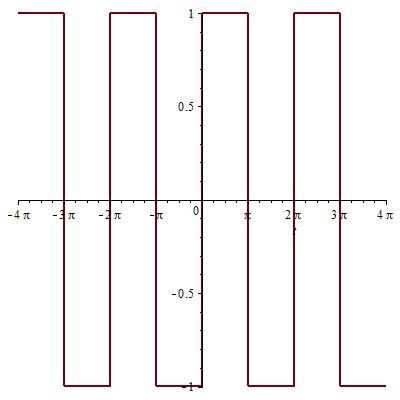
\includegraphics[height=30mm, width=60mm]{SquareWave.jpg}
\label{overflow}
\end{figure}

\begin{displaymath}
   f(x) = \left\{
     \begin{array}{lr}
       1, &(x \in [0, (2n+1)\pi)),\\
       -1, &(x \in [(2n+1)\pi, (2n+2)\pi)).
     \end{array}
   \right.
\end{displaymath}

\pause We want to approximate this function with a sum of sines and cosines.

\hfill

\pause We know already that $\sin(nx)$ and $\cos(nx)$ are $2 \pi$ periodic, just like this square wave. So this gives us some hope.

}


%Slide #5
\frame{
\frametitle{Fourier Series}

We want to think of each $2 \pi$ periodic function as being an infinite sum of sines and cosines, kind of like this:

\begin{displaymath}
f(x) = \frac{a_0}{2} + \sum\limits_{n=1}^\infty a_n \cos(nx) + b_n \sin(nx)
\end{displaymath}

\pause The above is kind of messy to handle, so instead of that, we use Euler's formula $e^{i\tha} = \cos(\tha) + i \sin(\tha)$ to write

\begin{displaymath}
f(x) = \sum\limits_{n=-\infty}^\infty c_n e^{-inx}
\end{displaymath}

where (if we take $b_0 = 0$) $c_n = \frac{a_n-ib_n}{2}$ if $n \geq 0$ and $c_n = \frac{a_n+ib_n}{2}$ if $n \leq 0$. 
}


%Slide #6
\frame{
\frametitle{Fourier Series}

So, given a function $f$, we need to find out what $c_n$ should be. 

\hfill

\pause Consider
\begin{displaymath}
\int\limits_0^{2\pi} f(t)e^{int} dt
\end{displaymath}

\pause
\begin{displaymath}
=\int\limits_0^{2\pi} \sum\limits_{j=-\infty}^\infty c_j e^{(n-j)it} dt
\end{displaymath}

\pause
Now, we note that if $k \neq 0$, 
\begin{displaymath}
\int\limits_0^{2\pi} e^{ikt} dt = 0
\end{displaymath}

 
}

\frame{
\frametitle{Fourier Series}

So, 
\begin{displaymath}
\int\limits_0^{2\pi} f(t)e^{int} dt = \int\limits_0^{2\pi} c_n e^0 = 2\pi c_n
\end{displaymath}

\pause Dividing by $2 \pi$, we get 
\begin{displaymath}
c_n = \frac{1}{2\pi} \int\limits_0^{2\pi} f(t)e^{int} dt 
\end{displaymath}

\pause Now, we call 
\begin{displaymath}
f(x) = \sum\limits_{n=-\infty}^\infty c_n e^{-inx}
\end{displaymath}
the Fourier Series of $f$.
}

\section[Square Wave]{Square Wave}

%Slide #7
\frame{
\frametitle{Revisiting the Square Wave}

\begin{figure}[ht!]
\centering
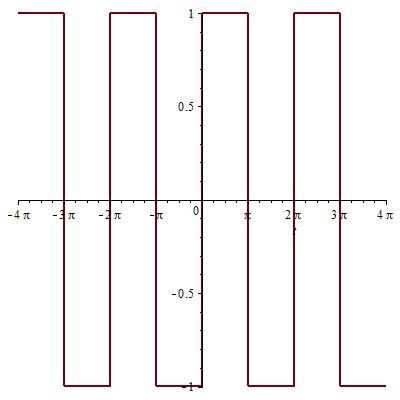
\includegraphics[height=25mm, width=60mm]{SquareWave.jpg}
\label{overflow}
\end{figure}

Doing this, we find that for the square wave,

\begin{displaymath}
   c_n = \left\{
     \begin{array}{lr}
       \frac{2i}{\pi n}, &(n $ is odd$),\\
       0, &(n $ is even$).
     \end{array}
   \right.
\end{displaymath}

\hfill

\pause So, the Fourier Series of the square wave is

\begin{displaymath}
f(x) = \sum\limits_{n=-\infty}^\infty \frac{2i}{\pi(2n+1)} e^{-(2n+1)ix} = \sum\limits_{n=-\infty}^\infty\frac{4}{\pi(2n+1)} \sin((2n+1) x)
\end{displaymath}

}

\frame{
\frametitle{More on the Square Wave}
It turns out that if we add up ``a lot'' of the terms of the Fourier Series, we get a good approximation.

\begin{figure}[ht!]
\centering
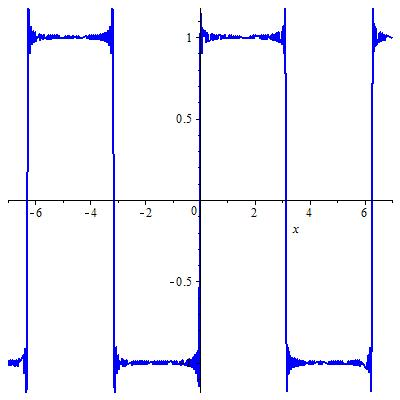
\includegraphics[height=25mm, width=60mm]{PartialSumFourierSeries.jpg}
\label{overflow}
\end{figure}

\pause That is, the square wave's Fourier Series converges to the square wave.

}

\section[Results]{Results}

\frame{
\frametitle{More on the Square Wave}

It turns out that if $f$ is periodic and piecewise smooth, then $f$'s Fourier Series converges to $f$, except at points of discontinuity.

\hfill

\pause Also, at a jump discontinuity occuring at $x$, $f$'s Fourier Series converges to

\begin{displaymath}
\frac{f(x^+) + f(x^-)}{2}
\end{displaymath}

\hfill

\pause That is incredibly nice.

}

\frame{
\frametitle{On to Other Functions}

So, we actually have that any smooth, periodic function has its Fourier Series converge to it.

\hfill

\pause That's incredibly useful; enough functions are smooth that knowing that the Fourier Series ``works'' is good.

\hfill

\pause This is very encouraging; we might want to extend this kind of result to any continuous, periodic function. 


}

\frame{
\frametitle{The Hope}

So, our hope is that we can prove the following theorem:

``Any periodic continuous function has its Fourier Series converge at each point. The Fourier Series of a function converges to the value of the function.''

}

\frame{
\frametitle{The Existence of a Continuous Function Whose Fourier Series Diverges at a Point}

Unfortunately, we can't do that.

\hfill

\pause We can show that there is a continuous, periodic function whose Fourier Series diverges at $0$.

\hfill

\pause In fact, we can construct a set of such functions that is dense in the set of continuous periodic functions.

\hfill

\pause That means we can approximate any continuous periodic function with a continuous periodic function whose Fourier Series diverges at $0$.

}



\frame{
\frametitle{The Existence of a Continuous Function Whose Fourier Series Diverges at a Point}

For brevity, let us say that given a periodic, continuous function $f$, $Mf = \sup(S_n(f,0))$, where $S_n(f,0)$ is the $n$th partial sum of $f$'s Fourier Series at $0$.

\hfill

\pause We construct for every real number, $A$, a continuous periodic function such that $\sup(|f(x)|) \leq 1$ and $Mf > A$

\hfill

\pause Then we consider the sets $E_n = \{f : Mf > n\}$. It turns out that these sets are open and dense. 

\hfill 

\pause The Baire Category Theorem says that in a complete metric space, the intersection of a collection of nonempty, open, dense sets is dense.

\hfill

\pause We use this to find a dense set of functions with $Mf = \infty$. 

}



\section[Acknowledgements]{Acknowledgements}
\frame{
\frametitle{Special Thanks}
I would like to thank:
\begin{itemize}
\item Dr. David C. Ullrich for his guidance and special brand of encouragement. 
\item Dr. Alan Noell for teaching me about Fourier Analysis.
\item The audience, for listening!
\end{itemize}
}



\end{document}






